\section{Design}
The design of the body is done with a  3D design software \href{https://www.freecadweb.org/}{Free-cad}. All part files are uploaded to the GitHub repository \url{https://github.com/tarragoesteve/TFM} under the hardware folder. You can see the main views on Figure \ref{fig:Isometric render view}, \ref{fig:Front render view}, \ref{fig:Top render view} and \ref{fig:Side render view}

We included three actuators in the robot because we want to control 3 degrees of freedom (inclination and speed of both wheels). Furthermore we introduced a fly-wheel to control the inclination of the body.  

We ensured symmetry along the axis formed by all motors in order to have an equilibrium in all possible inclinations without the need of external forces. We also took in consideration that the reinforcement learning algorithm starts being clumsy so none of the configurations should intersect with the ground. Figure \ref{fig:Side render view} illustrates this restriction.   

\begin{figure}
	\centering
	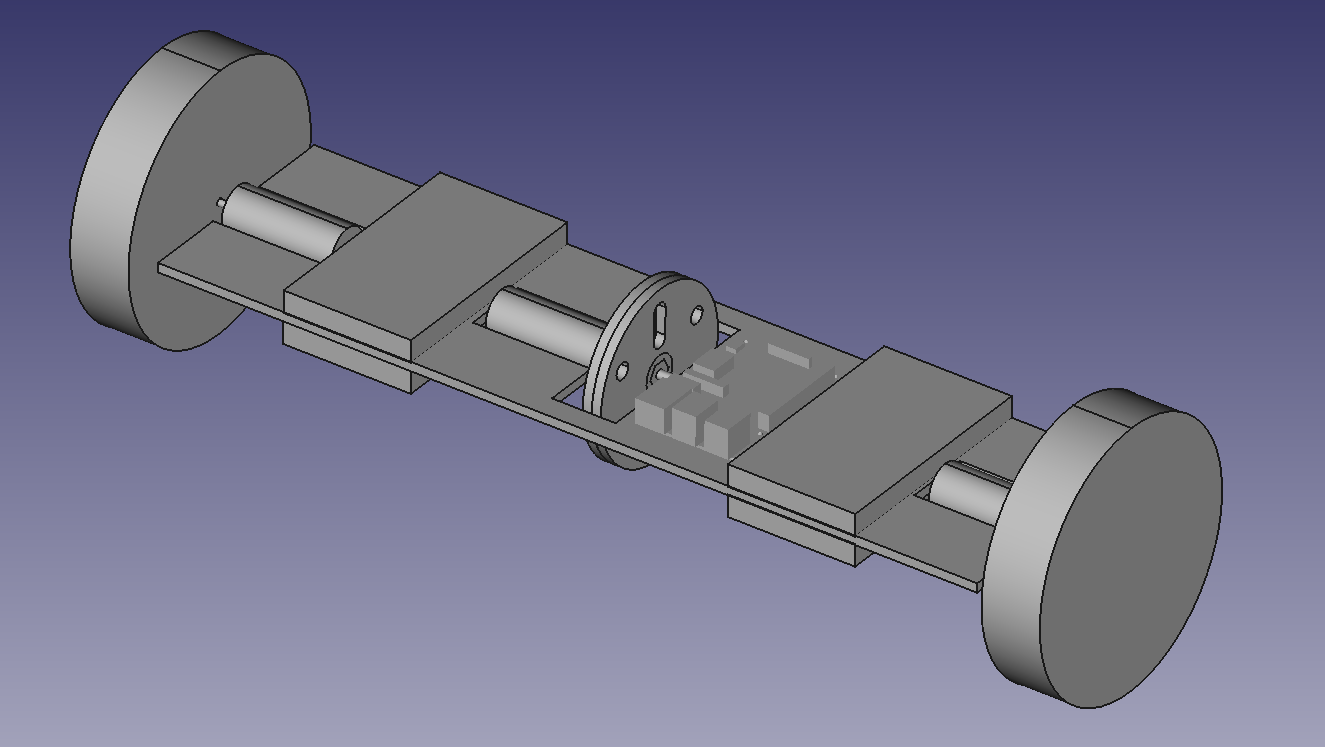
\includegraphics[width=10cm]{img/isometric_view.png}
	\caption{Isometric render view}
	\label{fig:Isometric render view}
\end{figure}
\begin{figure}
	\centering
	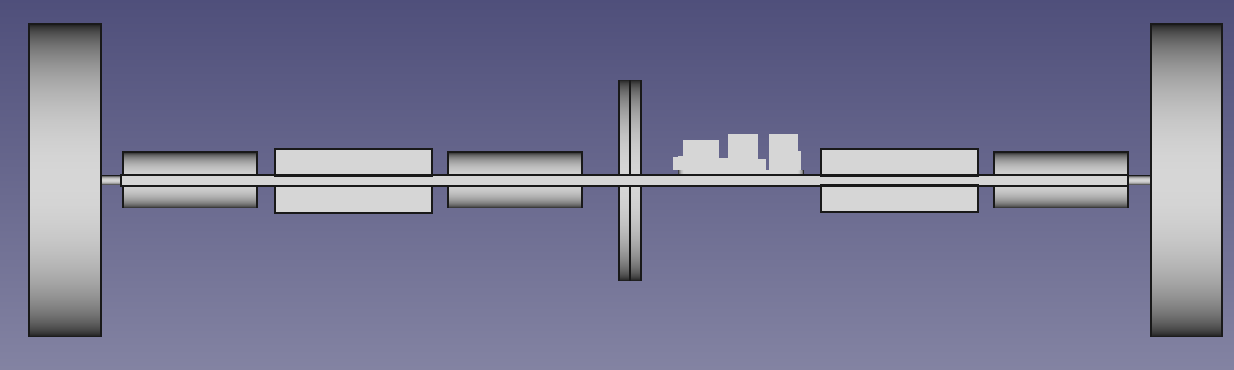
\includegraphics[width=10cm]{img/front_view.png}
	\caption{Front render view}
	\label{fig:Front render view}
\end{figure}
\begin{figure}
	\centering
	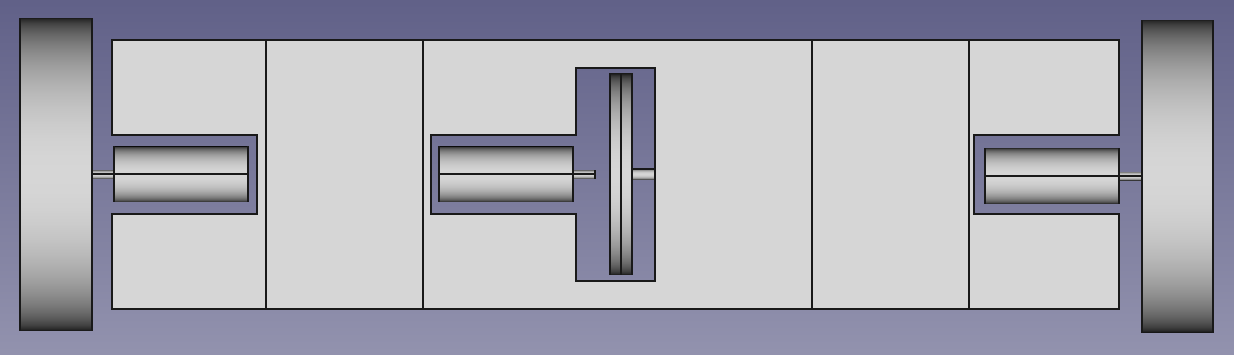
\includegraphics[width=10cm]{img/top_view.png}
	\caption{Top render view}
	\label{fig:Top render view}
\end{figure}
\begin{figure}
	\centering
	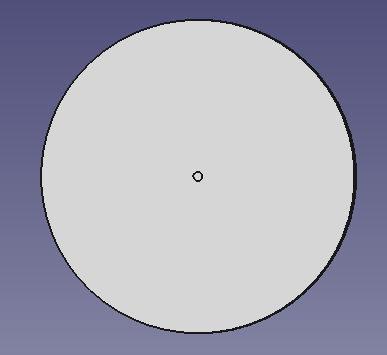
\includegraphics[width=4cm]{img/side_view.png}
	\caption{Side render view}
	\label{fig:Side render view}
\end{figure}

\subsection{Flywheel design}
\begin{figure}
	\centering
	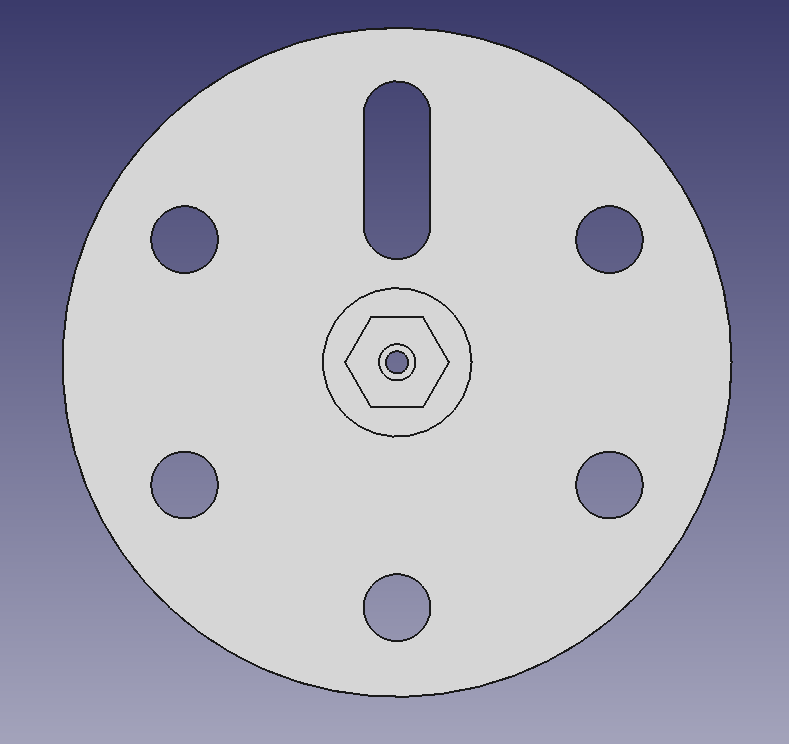
\includegraphics[width=5cm]{img/fly_wheel_side.png}
	\caption{Fly wheel side render view}
	\label{fig:Fly wheel side render view}
\end{figure}

To control the inclination of the body two strategies where taken in to account. Creating torque by a pendulum or by a the acceleration of flywheel. In order to experiment with both of them we designed a part to allow both configuration by placing weights in different spots, figure \ref{fig:Fly wheel side render view}.

One of the weight can be placed along a rail. The distance to the center will vary from $r_{min} = r_c + r_{motor-axis} \approx r_c $ to $r_{max} = r_f - r_c$. The pendulum torque $\tau$, considering the masses are cylinders of width $w$ and radius $r_c$, and the flywheel has a radius $r_f$ is the following:

Each mass weights:
\[ m = \rho * w * \pi * r_c^2 \]

All mass will be compensate the opposed one except the two with different radius.
The maximum torque takes place when these two masses are aligned horizontal with respect the ground and the movable weight is at distance $r_{min}$ from the center.

\[ \tau _{max} (r_c) = m * r_{max} - m * r_{min} = m * (r_f - 2 * r_c) \]

In order to maximize it we first compute the derivative:
\[\frac{\partial \tau _{max} (r_c)}{\partial r_c} = \frac{\partial m}{\partial r_c} * (r_f - 2 * r_c) - m * 2\]

\[ \frac{\partial m}{\partial r_c} = 2 * \rho * w * \pi *  r_c\]

An make it zero to find the maximum:

\[\frac{\partial \tau _{max} (r_c)}{\partial r_c} = 0\]

Substituting and simplifying we get:

\[\frac{\partial m}{\partial r_c} * (r_f - 2 * r_c) =  m * 2 \Rightarrow 2 * \rho * w * \pi *  r_c\ * (r_f - 2 * r_c) = \rho * w * \pi * r_c^2 * 2 \]

\[ \Rightarrow r_c\ * (r_f - 2 * r_c) =  r_c^2 \Rightarrow (r_f - 2 * r_c) =  r_c \Rightarrow r_f = 3 * r_c\]


The circumradius $R$ from the center of a regular polygon to one of the vertices is related to the side length $s$ by:

\begin{center}
	\begin{tabular}{ c  c }
		\(\displaystyle R=\frac {s}{2* \sin{\frac {\pi} {n}}} \)
		& 
		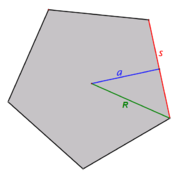
\includegraphics[width=3cm]{img/PolygonParameters.png}
	\end{tabular}
\end{center}

In our case:
\[ R = r_f - r_c; \]
\[ s = 2 * r_c\]

Substituting in the circumradius equation we get n = 6, so we will use 6 masses in our flywheel.